\documentclass[11pt,a4paper,oneside,german]{article}
\pagestyle{plain}
\usepackage[english]{babel}
\usepackage[utf8]{inputenc}

\usepackage{geometry}
\geometry{a4paper,left=40mm,right=30mm, top=3.5cm, bottom=2.5cm}
\usepackage{graphicx}
\usepackage{hyperref}

\title{Praktikumsbericht}
\author{Robin Mayer, Nils Nover, Mariella Zunker}
\date{\today}

\begin{document}
\maketitle

\newpage

\tableofcontents

\section{Fragestellung und Auswahl der Datensätze}

Die Frage der Schädlichkeit von Stickoxiden und deren Zusammenhang mit Dieselfahrzeugen hat in der Vergangenheit die Debatte um die Verkehrswende dominiert. Um einen Überblick über die Rolle von verschiedenen Antriebsarten zu bekommen, sollten in diesem Projekt Daten zu Antriebsdaten mit Stickoxidwerten in Deutschland verglichen werden. Hierbei sind einerseits die Unterschiede in verschiedenen Stadt- und Landkreisen zu berücksichtigen, auf der anderen Seite sollte auch die zeitliche Entwicklung und der lokale Einfluss von sogenannten Umweltzonen betrachtet werden. In Umweltzonen sind als nicht-schadstoffarm gekennzeichnete Fahrzeuge verboten, um die Luftqualität zu verbessern. \\
Zu Analyse der Fragestellung wurden Datensätze des Umweltbundesamtes [QUELLE] sowie des Kraftfahrtbundesamtes [QUELLE] genutzt. Die Datensätze des Umweltbundesamtes lagen als .xlx-Dateien vor und beinhalteten Informationen zu jahresgemittelten Stickoxidwerten an verschiedenen deutschen Messstationen(\ref{fig:BeispielNO2}), während das Kraftfahrtbundesamt hauptsächlich .pdf-Dateien veröffentlichte, in denen die zu einem Stichtag zugelassenen Anzahlen von Autos nach Antriebsart in den jeweiligen Orten aufgelistet waren (\ref{fig:BeispielKFZ}). Beide Quellen stellen Datensätze nach Jahr zu Verfügung.

\begin{figure}[h!]
	\centering
	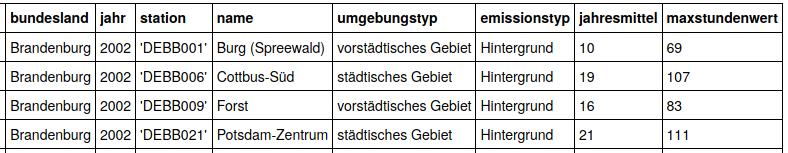
\includegraphics[width=10.5cm]{BeispielNO2.png}
	\caption{Auszug aus dem NO2-Datensatz.}
	\label{fig:BeispielNO2}
\end{figure}

\begin{figure}[h!]
	\centering
	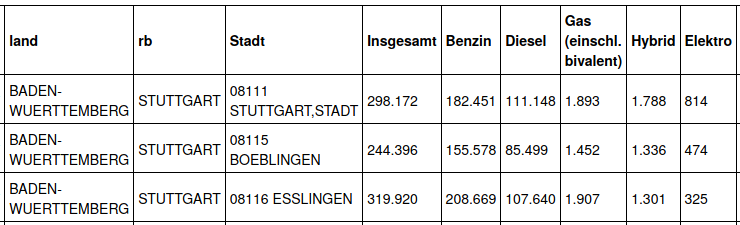
\includegraphics[width=10.5cm]{BeispielKFZ.png}
	\caption{Auszug aus dem KFZ-Datensatz.}
	\label{fig:BeispielKFZ}
\end{figure}

\section{Datenaufbereitung}

Zunächst mussten die Datensätze in ein Format konvertiert werden, in dem sie sinnvoll verarbeitet werden konnten. Dazu wurden zuächst die .pdf-Dateien ins .xslx-Format konvertiert. Aufgrund der großen Unterschiede der beiden Formate musste hierbei jedoch manuell noch viel nachgebessert werden (WAS?), weshalb nicht alle zur Verfügung stehenden Jahrgänge ausgewertet werden konnten. Die .xlsx-Dateien konnten im Anschluss in ein .csv-Format konvertiert und als solches eingelesen werden.\\
Aufgrund der guten Verfügbarkeit bestehender Tools und Libraries wurde für die Auswertung Python gewählt. Hierbei konnte vor allem auf das Datenanalysetool Pandas sowie Numpy und Matplotlib für die Auswertung zugegriffen werden. Das Jupyter Notebook stellt zudem eine übersichtliche und gut nachvollziehbare Programmierumgebung dar, in der Code gut im Team erarbeitet werden kann.\\
Nach dem Einlesen wurden die Datensätze auf Vollständigkeit und Fehler durchsucht. Dabei wurde auf nicht erfasste Datenpunkte sowie offensichtliche Abweichungen wie negative Zahlen geachtet. Zudem mussten die Städtenamen und alle als String codierten Variablen überprüft und vereinheitlicht werden. So wurden alle Namen in Großbuchstaben und ohne Umlaute dargestellt, sowie Rechtschreibfehler und Unterschiede in der Darstellung von Doppelnamen korrigiert. \\
Zudem wurden Messwerte, die keinem eindeutigen Ort zugewiesen werden konnten, aus dem Datensatz gelöscht, da eine nicht-automatisierte Zuordnung in der verfügbaren Zeit nicht möglich war.

\section{Datenauswertung}

Die Datensätze wurden zuerst isoliert betrachtet. Zur Messung der Luftwerte existierten Daten aus den Jahren 2002-2019. Die  Datensätze enthielten auch Zuordnungen der einzelnen Orte zu verschiedenen Abstufungen der Urbanität wie "vorstädtisches Gebiet". Die bestehende Einteilung wurde zur Vereinfachung zu den drei Kategorien "städtisch", "vorstädtisch" sowie "ländlich" zusammengefasst. Für einen ersten Überblick wurden die Stickoxidwerte über die Zeit geplottet (\ref{fig:NO2Entwicklung}).

\begin{figure}[h]
	\centering
	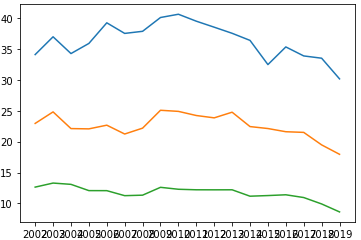
\includegraphics[width=10.5cm]{NO2Entwicklung.png}
	\caption{Entwicklung der Stickoxide über die Zeit. Blau: Städtisch. Gelb: Vorstädtisch. Grün: Ländlich.}
	\label{fig:NO2Entwicklung}
\end{figure}

\subsection{Vergleich der Stickoxidwerte zwischen den Bundesländern}

\subsection{Vergleich der Stickoxidwerte zwischen ausgewählten ländlichen und städtischen Gebieten}

\section{Interpretation der Ergebnisse}

\section{Diskussion}

\end{document}